\begin{figure}[t]
\centering
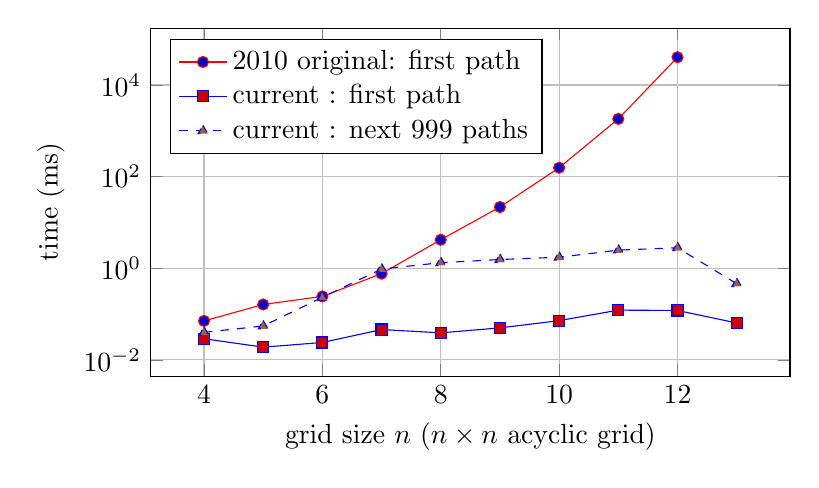
\begin{tikzpicture}
\begin{semilogyaxis}[width=0.8\textwidth,height=6cm,xlabel={grid size $n$ ($n\times n$ acyclic grid)},
  ylabel={time (ms)},legend pos=north west,grid=major,legend cell align=left]
\addplot+[mark=*,red] coordinates {(4,0.071) (5,0.162) (6,0.243) (7,0.764) (8,4.189) (9,21.712) (10,156.248) (11,1820.357) (12,40345.372)};
\addlegendentry{2010 original: first path}
\addplot+[mark=square*,blue] coordinates {(4,0.029) (5,0.019) (6,0.024) (7,0.046) (8,0.039) (9,0.05) (10,0.072) (11,0.122) (12,0.12) (13,0.064)};
\addlegendentry{current \cs{}: first path}
\addplot+[mark=triangle*,blue,dashed] coordinates {(4,0.04) (5,0.055) (6,0.232) (7,0.964) (8,1.323) (9,1.553) (10,1.741) (11,2.489) (12,2.797) (13,0.461)};
\addlegendentry{current \cs{}: next 999 paths}
\end{semilogyaxis}
\end{tikzpicture}
\caption{The 2010 implementation enumerates all $\binom{2(n-1)}{n-1}$ paths in the first query; the current one
computes one tree and then each path on demand.}
\label{fig:baseline}
\end{figure}
